\documentclass[a4paper,12pt]{article}

%\usepackage[latin1]{inputenc}
\usepackage[utf8]{inputenc}
\usepackage{amsfonts,amstext}
\usepackage{amssymb}
\usepackage{amsmath}
\usepackage{graphicx}
\usepackage[portuguese]{babel}
\usepackage{mathrsfs}
\usepackage[framed,numbered,autolinebreaks,useliterate]{mcode}
\usepackage[tbtags]{amsmath}

\newcommand{\R}{\mathbb{R}}

\begin{capa}
\vfill
\begin{center}
{\MakeUppercase{\Large Universidade de São Paulo -- USP}}\\
{\MakeUppercase{\large Escola de Engenharia de São Carlos}}\\
{\MakeUppercase{\large Departamento de Engenharia Elétrica}}\\
%{\MakeUppercase{\large Curso de Engenharia Elétrica}}
\vspace{6cm}

{\MakeUppercase{\large SEL0326 - Controle de sistemas lineares}} \\[3cm]  		% Escreva no lugar da palavra ''disciplina'' o nome da matéria
{\MakeUppercase {\Large  Trabalho }}\\[3cm]       % Escreva no lugar da palavra ''Título'' seu título
\end{center}

\begin{flushright}
      	\large	Guilherme Alves de Oliveira \\ NºUSP : 10748570
\end{flushright}

\end{capa}

\begin{document}

\newpage

\tableofcontents

\newpage

\section{Simulação MATLAB}

Para a realização deste trabalho foi desenvolvido o seguinte código anexado com a respectiva simulação no Simulink:

\begin{lstlisting}

clear all; close all; 
clc;
%%  ETAPA 1

A=  [    0      376.9911       0          0    ;
     -0.15685       0      -0.0784        0    ;
     -0.16725       0      -0.46296    0.166667;
     1572.825       0      -5416.98      -100 ];

B=  [    0          0          0        10000]';

da = zeros(4);
dp = zeros(4);

%---ETAPA 1.a)---%
%   Determinacao da matriz de incertezas
for i=1:4
    for j=1:4
        dp(i,j) = (0.05*rand(1)*(sign(0.5 - rand(1))));
        da(i,j) = A(i,j)*dp(i,j);
    end
end

dA= [    0          0          0          0    ;
      da(2,1)       0       da(2,3)       0    ;
      da(3,1)       0       da(3,3)    da(3,4) ;
      da(4,1)       0       da(4,3)       0   ];
  
%---ETAPA 3.b)---%
%   Determinacao da matriz nominal A+dA;
An = A + dA;                    

%%  ETAPA 2
Q = diag([0.1 0.1 0.01 0.00001]);   
R = [1];

%%  ETAPA 3
%---ETAPA 3.a)---%

[K, P, E] = lqr(An, B, Q, R);

%---ETAPA 3.b)---%

x0 = [0 0 0 0.1]';

%   Simulacao do modelo em simulink
out = sim('ModeloTrabalho');

%   Outputs da simulacao do modelo acima
t = out.X_out.time;             % Tempo
X = out.X_out.signals.values;   % Estados X
U = out.U_out.signals.values;   % Acao de controle U

%   Calculo do Funcional J
JD = X*Q*X' + U*R*U';
J = zeros(1,length(JD));
for i=1:(length(JD))
    J(1,i) = JD(i,i);
end
JI = trapz(t,J);

%   Calculo de X0T*P*X0
XP = x0'*P*x0;

%---ETAPA 3.c)---%

%   Determinacao das saidas x1, x2, x3 e x4 da simulacao
x1 = X(:,1);
x2 = X(:,2);
x3 = X(:,3);
x4 = X(:,4);

figure(1)       % Plot dos valores de X1
subplot(5,1,1)
plot(t,x1)
grid on 
legend('x_{1}')

subplot(5,1,2)  % Plot dos valores de X2
plot(t,x2)
grid on 
legend('x_{2}')

subplot(5,1,3)  % Plot dos valores de X3
plot(t,x3)
grid on 
legend('x_{3}')

subplot(5,1,4)  % Plot dos valores de X4
plot(t,x4)
grid on 
legend('x_{4}')

subplot(5,1,5)  % Plot dos valores da acao de controle U
plot(t,U)
grid on 
legend('u')

%%  ETAPA 4

JI2 = zeros(1,100);

%   Ciclo contendo os 100 novos sorteios para delta(a) e
%   o calculo do funcional J para cada novo sorteio.

for k=1:100
    %---ETAPA 4.a)---%
    %   Definicao dos A's nominais para cada sorteio
    for i=1:4
        for j=1:4
            dp(i,j) = (0.05*rand(1)*(sign(0.5 - rand(1))));
            da(i,j) = A(i,j)*dp(i,j);
        end
    end

    dA= [    0          0          0          0    ;
          da(2,1)       0       da(2,3)       0    ;
          da(3,1)       0       da(3,3)    da(3,4) ;
          da(4,1)       0       da(4,3)       0   ];

    An = A + dA;   
    
    %Simulacao com A nominal encontrado neste sorteio
    out = sim('ModeloTrabalho');
    t = out.X_out.time;
    X = out.X_out.signals.values;
    U = out.U_out.signals.values;
    
    %---ETAPA 4.b)---%
    JD = X*Q*X' + U*R*U';
    
    J2=zeros(1,length(JD));
    for i=1:(length(JD))
        J2(i) = JD(i,i);
    end
    JI2(k) = trapz(t,J2);
    
end

%---ETAPA 4.c)---%
figure(2)
k = 1:100;
plot(k,JI2)

\end{lstlisting}

\begin{figure}[!h]
  \vspace{3cm}
  \hspace*{0cm} 
  \includegraphics[width=15 cm]{ModeloSimulink.png}
  \centering
  \caption{Imagem contendo o modelo Simulink utilizado para simular o sistema em Espaço de Estados desenvolvido no Trabalho.}
  \label{Simulink}
\end{figure}

\clearpage

\section{ETAPA 1}
\subsection{Determinação da Matriz de Incertezas}
\label{subsec:matrizincerteza}

Para desenvolver a matriz de incertezas foi realizada a seguinte lógica. É feita um varredura de cada posição de uma matriz 4x4, para cada uma dessas posições foi sorteado um valor aleatório de variação entre $\pm 5\%$. Após determinar essa variação percentual é selecionado o elemento da Matriz A que possui a mesma posição desta variação e é feita a multiplicação entre esses valores. 

A lógica numérica que determina o valor dessas variações é a seguinte. Foi utilizado o comando $'rand(1)'$ cuja função é retornar um valor 'y' aleatório entre 0 e 1. Em seguida esse valor 'y' é multiplicado por 5 (como se estivesse sorteando um valor entre 0 e 5) e dividido por 100 (para se adquirir uma porcentagem). Logo em seguida é sorteado um valor 'x' entre $\pm 0.5$ e é utilizado o comando $'sign(x)'$, que retorna os valores -1, 0 ou 1 dependendo do sinal de x, esse valor multiplica '0.05y' encontrado anteriormente e determina o seu sinal. Gerando, assim, um número na faixa de $\pm 5\%$, cuja distribuição de probabilidade é uniforme. 


\begin{figure}[!h]
  \hspace*{-1cm} 
  \includegraphics[width=8 cm]{MatrizIncerteza.png}
  \centering
  \caption{Imagem contendo as variações percentuais de cada posição da Matriz de variações $dp$.}
  \label{MatrizdeVariacoes}
\end{figure}

\clearpage

\begin{figure}[!h]
  \hspace*{-1cm} 
  \includegraphics[width=8 cm]{MatrizDeltaAInicial.png}  
  \centering
  \caption{Imagem contendo o resultado da multiplicação entre os termos da Matriz da Figura \ref{MatrizdeVariacoes} e o elemento de mesma posição na Matriz A.}
  \label{MatrizDeltaINICIAL}
\end{figure}


Porém ainda não foi determinada a matriz $\Delta A$. Para isso, são selecionados alguns elementos da Matriz apresentada na Figura \ref{MatrizDeltaINICIAL}. Essa seleção é feita de acordo com o enunciado do trabalho (linha 25 do Código). Portanto a Matriz $\Delta A$ final é a seguinte:

\begin{figure}[!h]
  \hspace*{-1cm} 
  \includegraphics[width=8 cm]{MatrizDeltaA.png}
  \centering
  \caption{Imagem contendo a Matriz $\Delta A$}
  \label{MatrizDeltaA}
\end{figure}

\subsection{Determinação da Matriz Nominal do grupo}

Para determinar a Matriz Nominal (An) bastou apenas somar a Matriz A dado no enunciado pela matriz $\Delta A$ encontrada na Figura \ref{MatrizDeltaA}. O que gerou o seguinte resultado:

\begin{figure}[!h]
  \hspace*{-1cm} 
  \includegraphics[width=8 cm]{MatrizNominal.png}
  \centering
  \caption{Figura contendo a Matriz nominal, que será utilizada para desenvolvir as etapas 2 e 3 deste trabalho.}
  \label{MatrizNominal}
\end{figure}
\clearpage
\newpage

\section{ETAPA 2}
\subsection{Definição do Funcional LQR}

O problema apresentado no enunciado do trabalho não apresenta modelagem física explicita, ou seja, por mais que o mesmo tenha sido baseado em algum sistema físico real o mesmo não é explicitado no enunciado das questões. Diante disso, não é possível desenvolver uma lógica quantitativa/objetiva para escolher as matrizes Q e R. 

Diante disso, foram feitas algumas simulações alterando ambas as matrizes e as matrizes que foram escolhidas foram as seguintes:

$$
Q = \left(
\begin{array}{cccc}
0.1 &	0	& 0	& 0 \\
0&	0.1&	0&	0 \\
0&	0&	0.01&	0 \\
0&	0&	0&	1.0\cdot 10^{-5}  \\
\end{array}\right)
\text{ e } R=(1)
$$

\newpage

\section{ETAPA 3}
\subsection{Calculo do ganho ótimo K}
\label{subsec:GanhoK}

Para encontrar a matriz de ganho K que minimiza o funcional J dado pela equação 

$$ J = \int_{0}^{\infty} \left( x^T Q x + u^T R u\right) dt $$
foi utilizado o comando '$[K,P,E]=lqr(An,B,Q,R)$' do Matlab. Esse comando retorna a matriz de ganho 'K', a matriz solução da equação de Ricatti 'P' e a matriz de Autovalores do sistema 'E'.

Dadas as entradas An (matriz A + $\Delta A$ do modelo nominal), B, Q e R, o comando '$lqr$' realiza as seguintes operações:
\begin{itemize}
    \item Encontra P resolvendo a Equação de Ricatti
    $$ A^T P + PA + PBR^{-1}B^TP + Q = 0$$
    \item Encontra K Substituindo P encontrado no item anterior na seguinte expressão
    $$ K = R^{-1}B^TP $$
    \item Encontra E calculando os autovalores de $\left(A-BK\right)$
\end{itemize}

\begin{figure}[!h]
  \hspace*{-1cm} 
  \includegraphics[width=8 cm]{PRicatti.png}
  \centering
  \caption{Figura contendo a matriz P encontrada a partir solução da equação de Ricatti para as matrizes An, B, Q e R definidas anteriormente.}
  \label{PRiccati}
\end{figure}
\clearpage
\begin{figure}[!h]
  \hspace*{-1cm} 
  \includegraphics[width=8 cm]{MatrizganhoK.png}
  \centering
  \caption{Matriz de ganho ótimo K encontrada a partir da matriz P da Figura \ref{PRiccati}.}
  \label{GanhoK}
\end{figure}

\subsection{Cálculo do funcional J}
\label{subsec:FuncJ}

Para encontrar o valor do funcional J para o ganho K da Figura \ref{GanhoK}, foi utilizado o modelo em Simulink apresentado na Figura \ref{Simulink}. A partir da simulação do modelo é possível resgatar os valores das variáveis de estados $x_i(t)$ e ação de controle $u(t)$. Após resgatar os valores de $x$ e $u$ foi feita a seguinte operação:

$$ x^T Q x + u^T R u = $$
$$
\left(
\begin{array}{cccc}
    x_1(0) & x_2(0) & x_3(0) & x_4(0) \\
    x_1(t_1) & x_2(t_1) & x_3(t_1) & x_4(t_1) \\
    \vdots & \vdots & \vdots & \vdots \\
    x_1(t_N) & x_2(t_N) & x_3(t_N) & x_4(t_N) \\
\end{array}\right) \cdot
Q \cdot
\left(
\begin{array}{cccc}
    x_1(0) & x_1(t_1) & \hdots & x_1(t_N) \\
    x_2(0) & x_2(t_1) & \hdots & x_2(t_N) \\
    x_3(0) & x_3(t_1) & \hdots & x_3(t_N) \\
    x_4(0) & x_4(t_1) & \hdots & x_4(t_N) \\
\end{array}\right) + \hdots

\hdots + 
\left(
\begin{array}{c}
     u(0)  \\
     u(t_1) \\
     \hdots \\
     u(t_N)
\end{array}
\right) \cdot R \cdot
\left(
\begin{array}{cccc}
   u(0)  & u(t_1) & \hdots & u(t_N) \\
\end{array}\right) =
$$

\scriptsize{
\begin{equation}
\left(
\begin{array}{cccc}
  \sum_{i=1}^{4} Q_i\cdot (x_i(0))^2 + R\cdot (u(0))^2    &                              0 &      \hdots & 0 \\
  0                                  & \sum_{i=1}^{4} Q_i\cdot (x_i(t_1))^2 + R\cdot (u(t_1))^2  &       \hdots      & \vdots  \\
  \vdots                             &                \vdots                    & \ddots      & 0 \\
  0                                  &                            \hdots  &           0 & \sum_{i=1}^{4} Q_i\cdot (x_i(t_N))^2 + R\cdot (u(t_N))^2\\
\end{array}\right)\normalsize
\label{MDQ}
\end{equation}}

\normalsize

A matriz encontrada na Equação \ref{MDQ} apresenta em sua diagonal principal os valores da função $J'(t)$ em cada instante $t_i$ simulado pelo modelo da Figura \ref{Simulink}. Para calcular o funcional J, portanto, foi preciso calcular a integral

$$ J \approx \int_{0}^{t_N}J'(t)dt $$

Para calcular um valor aproximado de J, foi utilizado um método de integração numérica, visto que não foi calculada uma função elementar para $J'(t)$. O método utilizado foi a integração trapezoidal e o tempo de simulação foi $t_N = 6$ segundos. O comando utilizado para implementar esse método foi o $'trapz(t,J)'$, onde $t$ é a matriz com os tempos $t_i$'s simulados e $J$ a matriz com os valores de $J'(t_i)$.

\begin{figure}[!h]
  \hspace*{-1cm} 
  \includegraphics[width=4 cm]{FuncionalJ.png}
  \centering
  \caption{Figura contendo o valor aproximado do Funcional J, encontrada partir da integração trapezoidal da função $J'(t)$.}
  \label{FuncionalJ}
\end{figure}

Encontrado o valor de J, agora é preciso calcular o valor da expressão 

\begin{equation}
 x_{0}^{T}\cdot P\cdot x_{0} \text{, onde } x_{0} = [\begin{array}{cccc}
   0  &  0 & 0 & 0.1\\
\end{array}]^T.\label{XTPX}\end{equation}

\begin{figure}[!h]
  \hspace*{-1cm} 
  \includegraphics[width=4 cm]{X0TPX0.png}
  \centering
  \caption{Figura contendo o valor encontrado para a Equação \ref{XTPX}. }
  \label{XPX}
\end{figure}

Após analisar o valor do funcional J e da expressão $x_{0}^{T}\cdot P\cdot x_{0}$ nas Figuras \ref{FuncionalJ} e \ref{XPX}, respectivamente, foi possível perceber que ambos apresentam valores muito próximos um do outro, com um pequena diferença de aproximadamente $2.7\%$.

\clearpage

\subsection{Resposta do modelo nominal em Malha Fechada}

Para plotar os gráficos das respostas no tempo $x_1 (t)$ a $x_4 (t)$ e $u(t)$ foram utilizados, novamente, os dados da simulação em Simulink da Figura \ref{Simulink}. A respostas dos estados do modelo nominal foram as seguintes:

\begin{figure}[!h]
  \hspace*{-2.4cm} 
  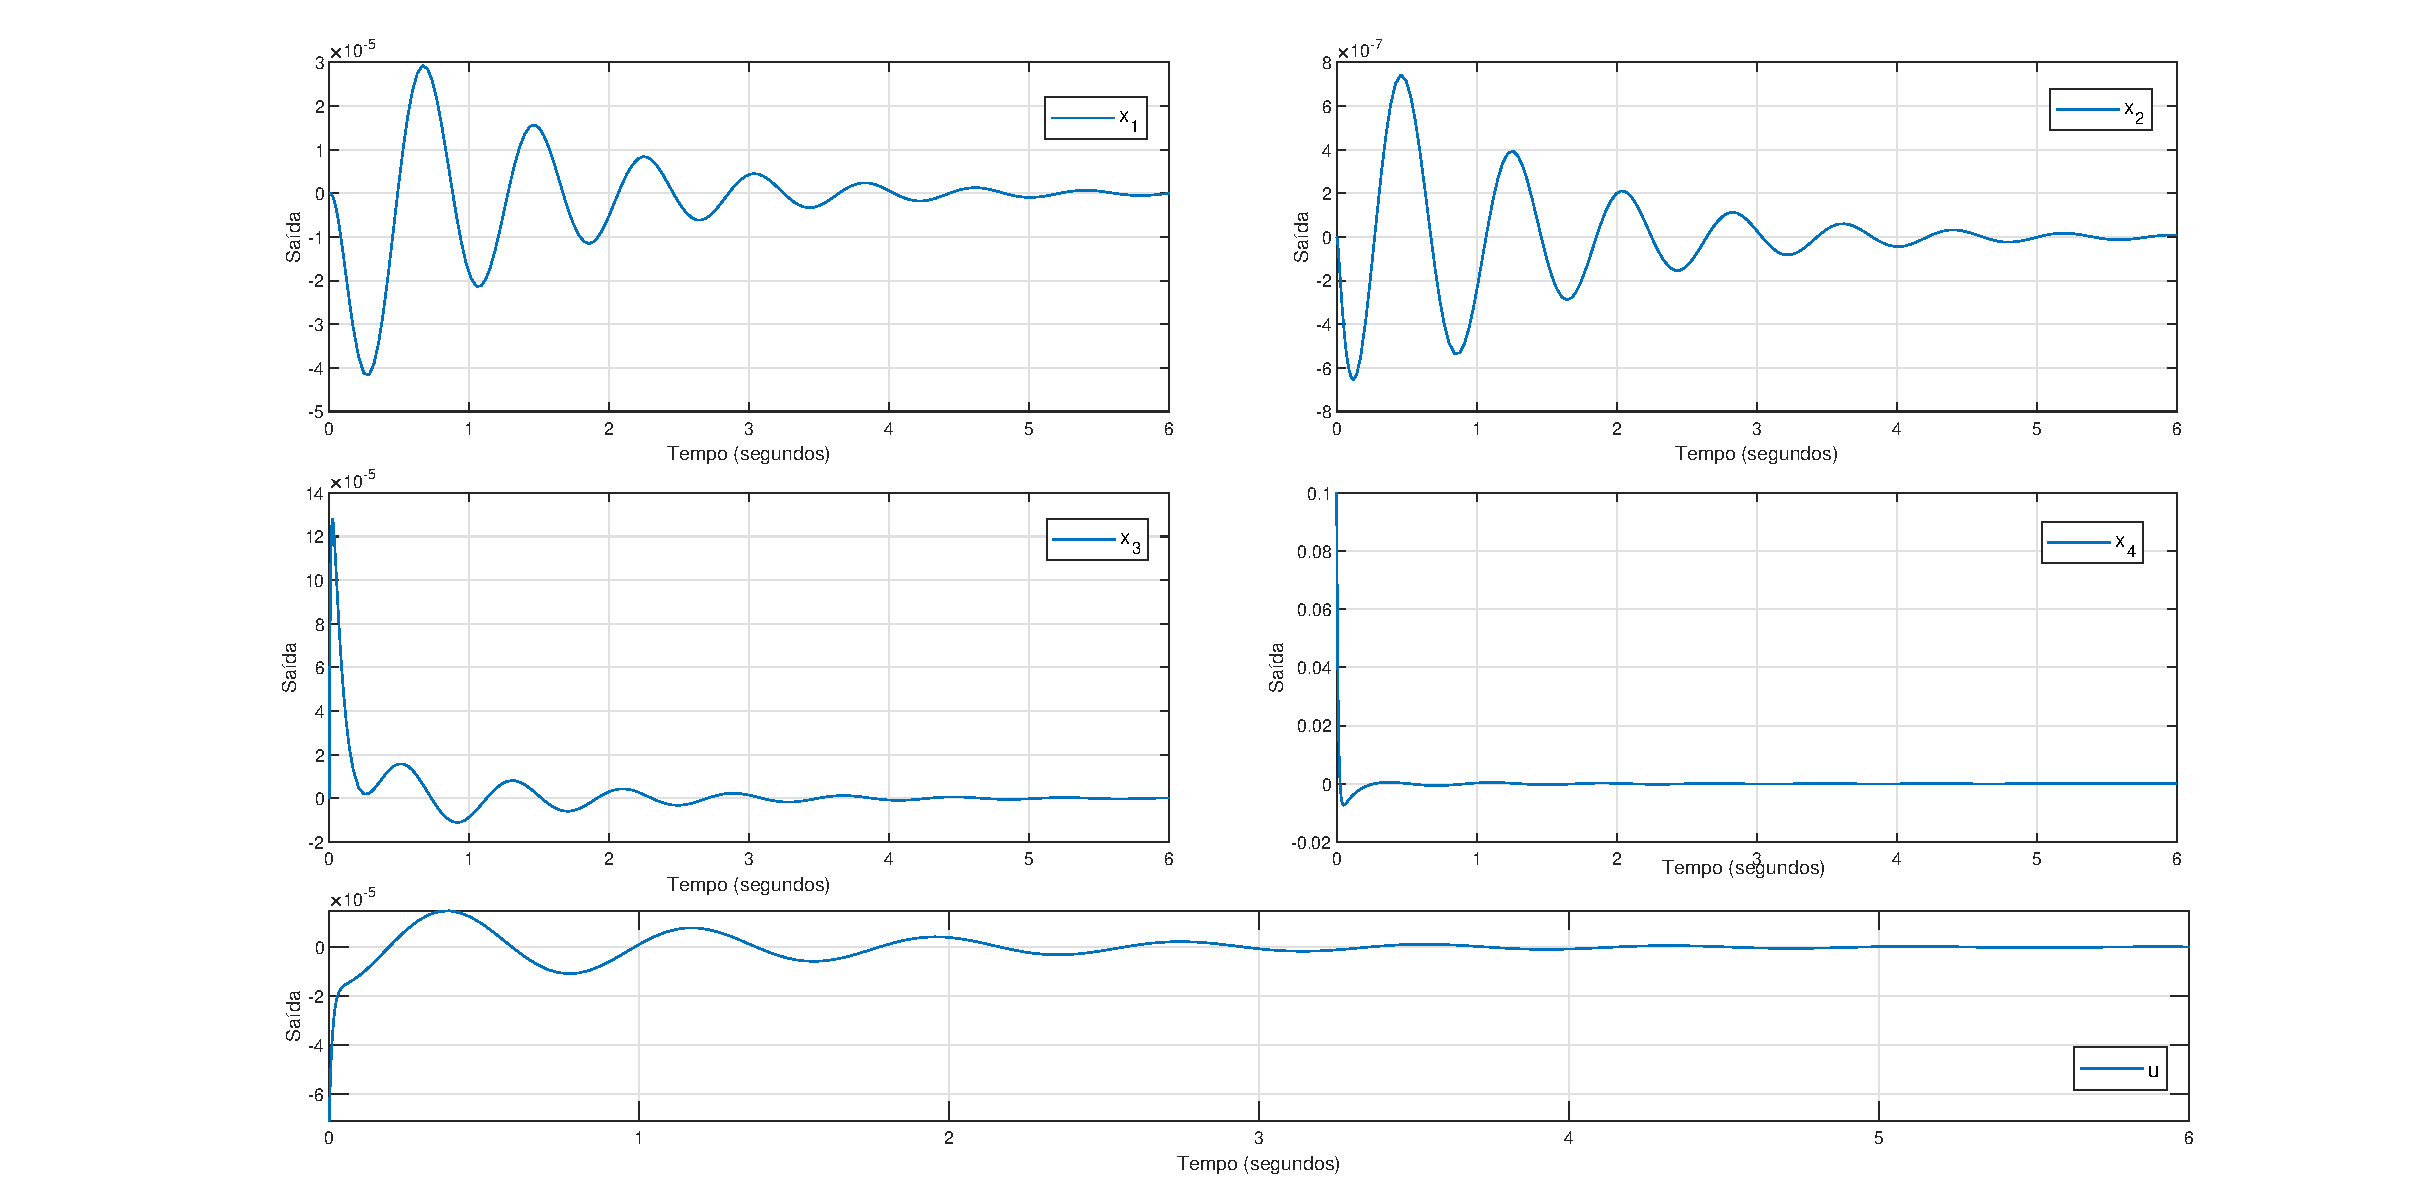
\includegraphics[width=18 cm]{SaidasEstadoseAcao.eps}
  \centering
  \caption{Figura contendo os Estados $x_1(t)$,$x_2(t)$,$x_3(t)$ e $x_4(t)$ e a ação de controle $u(t)$ do sistema nominal.}
  \label{EstadosAcao}
\end{figure}

\newpage

\section{ETAPA 4}
\subsection{Sorteios de $\Delta{a_{ij}}$}

Para a realização dos 100 novos sorteios de $\Delta{a_{ij}}$ foi utilizado o mesmo algoritmo da subseção \ref{subsec:matrizincerteza}, porém agora ele estará dentro de um laço '$for$', que rodará 100 ciclos deste algoritmo de formação da matriz de incertezas $\Delta A$. A cada ciclo é formado um novo modelo 'não-nominal', porém, será utilizada a matriz de Ganho K encontrada na subseção \ref{subsec:GanhoK}.

\subsection{Funcional J}

Para essa etapa também será calculado o valor do funcional J para cada um dos 100 modelos não-nominais do laço '$for$'. O algoritmo para encontrar o valor de J é exatamente igual ao da subseção \ref{subsec:FuncJ}. Todos os J's calculados nesta etapa estão dispostos no gráfico a seguir:

\begin{figure}[!h]
  \hspace*{-1cm} 
  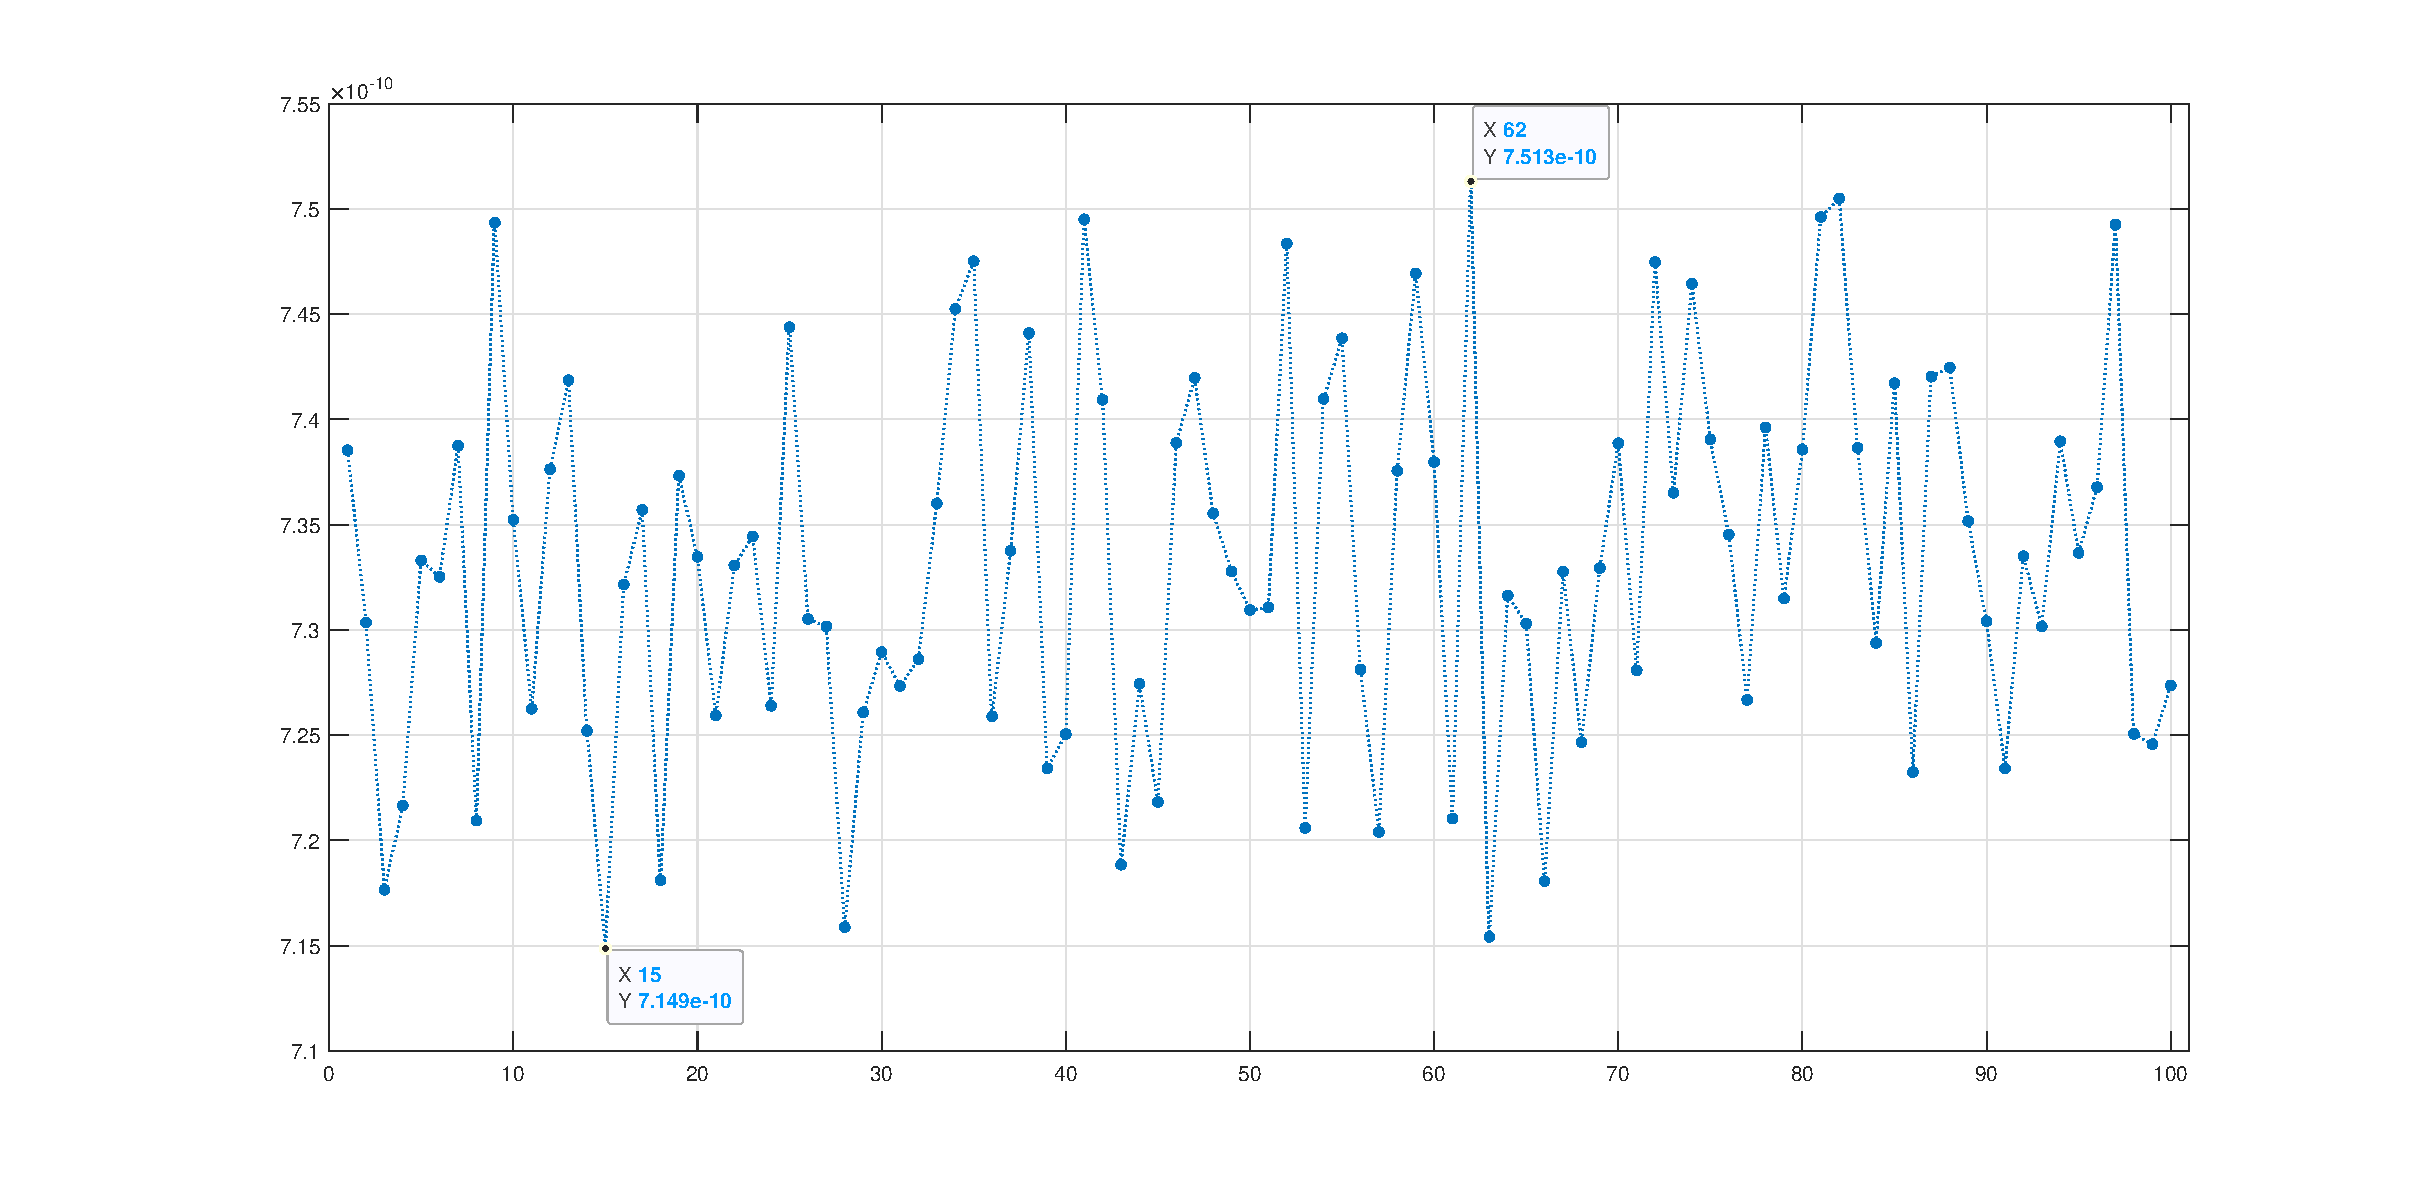
\includegraphics[width=15 cm]{J100.eps}
  \centering
  \caption{Gráfico contendo os valores do funcional J para cada um dos 100 modelos não-nominais.}
  \label{100J}
\end{figure}

Para analisar o efeito das incertezas na matriz de Estados sobre a otimalidade do controle LQR, foi utlizada a Figura \ref{100J} como base. A partir desta Figura foi feito o cálculo do erro/variação percentual do funcional J do modelo nominal ($7.294\cdot 10^{-10}$) e os valores máximo ($ 7.513\cdot 10^{-10}$) e mínimo ($7.149\cdot 10^{-10}$) dos funcionais J obtidos a partir das 100 simulações. 

\begin{equation}
    E_{MÁX} = 3.00\% \text{\hspace{0.8cm} e \hspace{0.8cm}} E_{MÍN} = -1.98\%
    \label{erros}
\end{equation}  

A partir dos resultados obtidos em \ref{erros}, foi possível perceber que, para o modelo de controle LQR, as incertezas na matriz de Estados influenciam de forma explícita no valor do funcional J. Isto é, para um sistema com uma mesma matriz de controle K, as variações nos parâmetros da matriz 'A' deste mesmo sistema em cada simulação geraram variações no valor do seu funcional J.

Portanto, pode-se perceber que a otimalidade do controle LQR não prevê as variações ou incertezas na matriz de estados.Para situações diferentes da matriz $\Delta A$ seria necessário encontrar uma nova matriz de controle K para otimizar o sistema. Ou seja, de modo geral, o controle LQX otimiza um sistema específico e muito bem definido. Quando o sistema sofre variações, esse controle, deixa de ser ótimo. 


\end{document}

\begin{figure}[!h]
  \hspace*{-1cm} 
  \includegraphics[width=15 cm]{  }
  \centering
  \caption{  }
  \label{  }
\end{figure}